% Appendix A: FAIR principles implementation
\section{FAIR principles implementation}
\label{app:fair}

The giveadam project implements all four FAIR principles \cite{wilkinson2016fair} through its semantic layering methodology and automated observability framework detailed in Section~\ref{sec:semantic-methodology}. This section demonstrates how the semantic approach enhances traditional FAIR compliance by making research processes themselves findable, accessible, interoperable, and reusable.

\subsection{Findable: Discovery and identification}

\textbf{Rich metadata and identifiers:} The datasets are published with comprehensive metadata in \texttt{data/README.md}, including detailed column descriptions, data provenance, and research context. Each dataset has unique identifiers (\texttt{respondents.csv}, \texttt{SDG\_rankings.csv}, \texttt{SDG\_labels.csv}, \texttt{SDG7\_analysis.csv}) and is version-controlled in the GitHub repository \texttt{giveadam} at \texttt{https://github.com/softloud/giveadam}.

\textbf{Semantic documentation:} Unlike standard data repositories, the semantic layering approach provides findable documentation at multiple conceptual levels. Researchers can locate relevant transformations by research concept (semantic models in Table~\ref{tab:dbt_models}) rather than technical implementation details. The four-layer architecture shown in Figure~\ref{fig:dbtdag} enables discovery through conceptual navigation.

\textbf{Automated cataloging:} The observability framework generates searchable metadata from pipeline artifacts (Table~\ref{tab:dbt_models}), ensuring that all data transformations and quality checks are discoverable through the automated documentation system detailed in Section~\ref{subsec:obs-table-gen}.

\subsection{Accessible: Retrieval and usability}

\textbf{Open access and standard protocols:} Data are published in universally accessible CSV format \cite{csv_rfc} without authentication barriers. The complete repository is openly available via HTTPS and Git protocols \cite{git}, supporting both web browser access and programmatic retrieval through GitHub \cite{github}.

\textbf{Human and machine readable:} Column names follow interpretable conventions prioritizing domain understanding over technical convenience. The semantic layer architecture (Figure~\ref{fig:dbtdag}) ensures that data structure reflects research logic rather than processing efficiency.

\textbf{Multiple access modalities:} Researchers can access data through multiple pathways: direct CSV download, Git repository cloning \cite{git}, or programmatic URL access in R \cite{r_core} or Python \cite{python}. The interactive dbt documentation (\texttt{dbt docs serve}) \cite{dbt_core} provides a web-based interface for exploring complete data lineage.

\subsubsection{SDG rankings dataset}

This dataset contains respondent rankings enriched with demographic metadata:
\begin{itemize}
  \item \textbf{id\_respondent:} Unique identifier for each respondent
  \item \textbf{rank:} Priority ranking (1=highest, 2=medium, 3=lowest priority)
  \item \textbf{sdg\_number:} UN SDG number (1-17)
  \item \textbf{sdg\_label:} Full name of the Sustainable Development Goal
  \item \textbf{age:} Age of respondent in years
  \item \textbf{gender:} Self-reported gender
  \item \textbf{displacement\_status:} Dam impact classification
  \item \textbf{region:} Survey location (tehri, arunachal)
\end{itemize}

By enriching the responses with respondent metadata, we can analyse responses in the context of respondent demographics and characteristics. For example, in Figure~\ref{fig:top3-gender-treemap}, we can see the distribution of top 3 UN SDG priorities by gender.

\begin{figure}[ht]
  \centering
  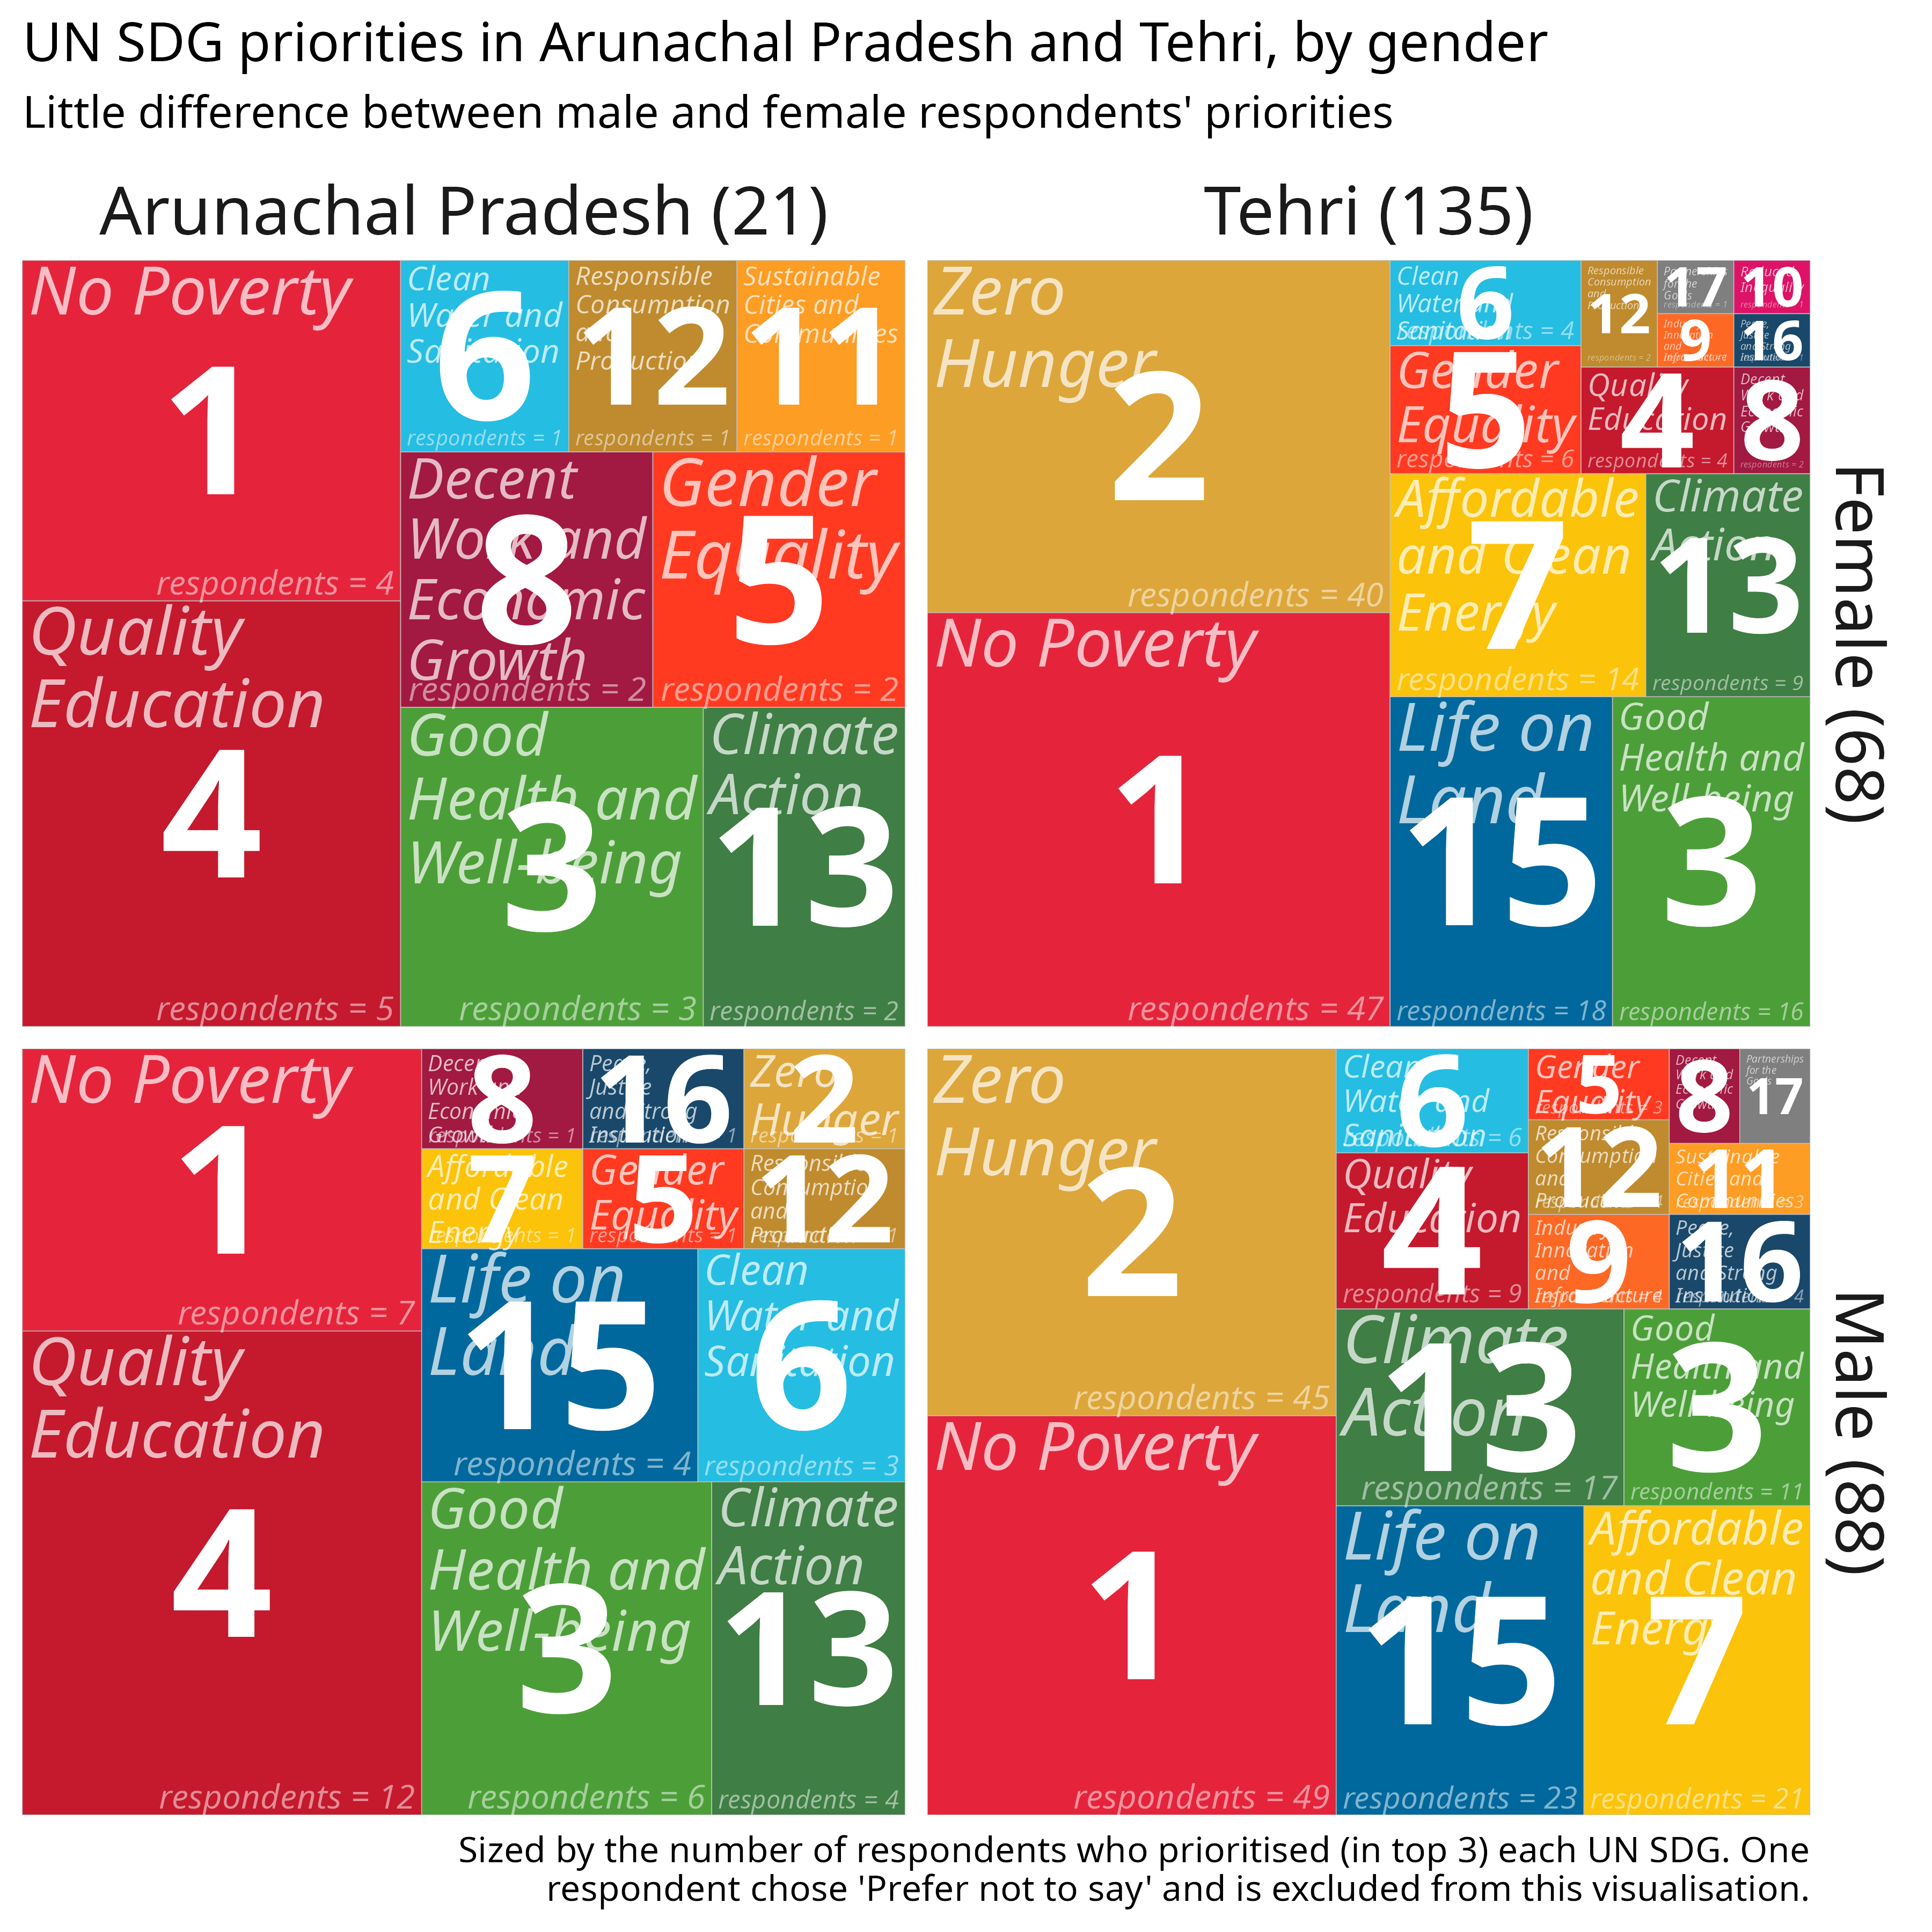
\includegraphics[width=0.95\textwidth]{../figures_and_tables/top3-gender-treemap.png}
  \caption{\label{fig:top3-gender-treemap} Treemap of top 3 UN SDG priorities from survey respondents in Tehri and Arunachal Pradesh, North India, by gender. Each rectangle represents a specific UN SDG, with its size proportional to the number of respondents of a particular gender who ranked it among their top three priorities. The treemap visually highlights the most and least prioritized SDGs in each region, providing insights into gender differences in development priorities.}
\end{figure}

\subsubsection{Respondents dataset}

\begin{itemize}
  \item \textbf{id\_respondent:} Unique identifier for each respondent
  \item \textbf{age:} Age of respondent in years
  \item \textbf{gender:} Self-reported gender (Male, Female, Prefer not to say)
  \item \textbf{displacement\_status:} Impact classification related to dam construction
  \item \textbf{region:} Survey location (tehri, arunachal)
\end{itemize}

\subsubsection{SDG labels dataset}

This reference dataset provides standardized UN Sustainable Development Goal identifiers and labels:
\begin{itemize}
  \item \textbf{sdg\_id:} Standardized identifier (e.g., "SDG\_1", "SDG\_2")
  \item \textbf{sdg\_number:} UN SDG number (1-17)
  \item \textbf{sdg\_label:} Full name of the Sustainable Development Goal
\end{itemize}

\subsubsection{SDG7 analysis dataset}

This analysis-ready dataset focuses on energy priorities (SDG 7: Affordable and Clean Energy):
\begin{itemize}
  \item \textbf{id\_respondent:} Unique identifier linking to respondents table
  \item \textbf{region:} Survey location (tehri, arunachal)
  \item \textbf{age:} Age of respondent in years
  \item \textbf{gender:} Self-reported gender
  \item \textbf{displacement\_status:} Dam impact classification
  \item \textbf{displacement\_group:} Grouped displacement categories for analysis
  \item \textbf{sdg\_7\_chosen:} Binary indicator (1 = SDG 7 in top 3, 0 = not in top 3)
\end{itemize}

This dataset enables focused analysis of energy priorities across demographic groups and displacement categories, supporting research into how dam construction impacts community energy preferences.

\subsection{Interoperable: Integration and exchange}

\textbf{Standard data formats and vocabularies:} Data are published in CSV format \cite{csv_rfc} using UTF-8 encoding with standardized missing value representation (NA). Column naming follows consistent conventions across datasets, enabling seamless joining and integration across the semantic layers shown in Figure~\ref{fig:dbtdag}.

\textbf{Semantic harmonization documentation:} The semantic layer explicitly addresses interoperability challenges by documenting how disparate data sources are harmonized. For example, SDG labeling differences between regional surveys are reconciled with full documentation of mapping decisions in the semantic models (Table~\ref{tab:dbt_models}), enabling other researchers to understand and adapt the harmonization logic.

\textbf{Modular pipeline architecture:} The dbt project structure (Section~\ref{sec:repository-arch}) separates concerns across semantic layers, enabling selective reuse of transformation logic. Researchers can adopt the source entity patterns for context preservation while modifying semantic harmonization for different research domains. Each semantic layer (Table~\ref{tab:dbt_models}) implements specific interoperability functions that can be independently understood and modified.

\textbf{Cross-tool compatibility:} Tidy data principles ensure compatibility across analytical software. The semantic layer structure provides conceptual interoperability—researchers can understand and adapt the methodology regardless of their technical implementation preferences.

\subsection{Reusable: Extension and adaptation}

\textbf{Comprehensive provenance and documentation:} Complete methodology documentation enables confident reuse across research contexts. The automated observability system (Section~\ref{subsec:obs-table-gen}) ensures that documentation evolves with implementation, preventing methodology drift that undermines reusability.

\textbf{Extensible semantic framework:} The semantic layering methodology provides a reusable framework beyond this specific dataset. The four-layer architecture (source base → source entities → semantic → analytic) demonstrated in Figure~\ref{fig:dbtdag} can be adapted for any multi-source research data integration challenge.

\textbf{Quality assurance infrastructure:} The validation framework (Table~\ref{tab:dbt_tests}) provides reusable patterns for data quality verification across research contexts. These automated tests ensure that reused components maintain data integrity standards.

\textbf{Licensing and attribution:} Data are licensed under Creative Commons Attribution 4.0 International (CC BY 4.0) \cite{creative_commons}, enabling broad reuse with appropriate attribution. The license covers both datasets and methodology, encouraging adaptation of the semantic layering approach.

\textbf{Technical infrastructure reusability:} The repository can be forked and the dbt pipeline extended for new data sources or research questions. The modular structure supports iterative development—researchers can extend the analytic layer for new questions without modifying upstream transformations.

\textbf{Methodological transferability:} The semantic layering approach addresses fundamental challenges in research data management that extend beyond this specific domain. The methodology's emphasis on context preservation, transparent harmonization, and stakeholder communication applies to any research requiring multi-source data integration and methodological transparency.